\documentclass{article}
\usepackage{fontspec}
\newfontfamily\hebrewfont[Script=Hebrew]{Calibri}
\usepackage[left=2.0cm, top=2.0cm, right=2.0cm, bottom=2.0cm]{geometry}
\usepackage{polyglossia}
\usepackage{amsmath}
\usepackage{listings}
\usepackage{color}
\usepackage{relsize}
\usepackage{graphicx}
\usepackage{bidi}

\setdefaultlanguage{english}
\setotherlanguage{hebrew}
\title{מטלת מנחה 14 - קורס 20277}
\author{328197462}
\date{04/09/2023}

\definecolor{gray}{rgb}{0.4,0.4,0.4}
\definecolor{darkblue}{rgb}{0.0,0.0,0.6}
\definecolor{cyan}{rgb}{0.0,0.6,0.6}
\definecolor{delim}{RGB}{20,105,176}
\definecolor{numb}{RGB}{106, 109, 32}
\definecolor{string}{rgb}{0.64,0.08,0.08}

\lstset{
  columns=fullflexible,
  showstringspaces=false,
  commentstyle=\color{gray}\upshape
}

\lstdefinelanguage{XML}
{
  morestring=[b]",
  morestring=[s]{>}{<},
  morecomment=[s]{<?}{?>},
  stringstyle=\color{black},
  identifierstyle=\color{cyan},
  keywordstyle=\color{cyan},
  morekeywords={}% list your attributes here
}

\lstdefinelanguage{N3}
{
  morestring=[b]",
  stringstyle=\color{cyan}
}

\lstdefinelanguage{JSON}{
    numberstyle=\small,
    rulecolor=\color{black},
    showspaces=false,
    showtabs=true,
    breaklines=true,
    postbreak=\raisebox{0ex}[0ex][0ex]{\ensuremath{\color{gray}\hookrightarrow\space}},
    breakatwhitespace=true,
    upquote=true,
    morestring=[b]",
    stringstyle=\color{cyan},
    literate=
     *{0}{{{\color{numb}0}}}{1}
      {1}{{{\color{numb}1}}}{1}
      {2}{{{\color{numb}2}}}{1}
      {3}{{{\color{numb}3}}}{1}
      {4}{{{\color{numb}4}}}{1}
      {5}{{{\color{numb}5}}}{1}
      {6}{{{\color{numb}6}}}{1}
      {7}{{{\color{numb}7}}}{1}
      {8}{{{\color{numb}8}}}{1}
      {9}{{{\color{numb}9}}}{1}
      {\{}{{{\color{delim}{\{}}}}{1}
      {\}}{{{\color{delim}{\}}}}}{1}
      {[}{{{\color{delim}{[}}}}{1}
      {]}{{{\color{delim}{]}}}}{1},
}

\lstdefinelanguage{SPARQL}{
  columns=fullflexible,
  breaklines=false,
  sensitive=true,
  % --------------------------
  xleftmargin=.5em,
  xrightmargin=.5em,
  framexleftmargin=.5em,
  framextopmargin=.5em,
  framexbottommargin=.5em,
  framexrightmargin=.5em,
  % --------------------------
  tabsize = 2,
  showstringspaces=false,
  morecomment=[l][\color{gray}]{\#},       % comments
  morestring=[b][\color{cyan}]{\"},  % strings
  % -------------------------- variables
  keywordsprefix=?,
  classoffset=0,
  keywordstyle=\color{delim},
  morekeywords={},
  % -------------------------- prefixes
  classoffset=1,
  keywordstyle=\color{cyan},
  morekeywords={rdf,rdfs,owl,xsd,purl},
  % -------------------------- keywords
  classoffset=2,
  keywordstyle=\color{cyan},
  morekeywords={
    select,CONSTRUCT,DESCRIBE,ASK,where,FROM,NAMED,PREFIX,BASE,OPTIONAL,
    FILTER,GRAPH,LIMIT,OFFSET,SERVICE,UNION,EXISTS,NOT,BINDINGS,MINUS,a
  }
}

\begin{document}

\begin{hebrew}
    \maketitle
    \section*{שאלה 1}

    \subsection*{סעיף א}
    המידע בהצגת XML ייראה כך:
\end{hebrew}

\begin{lstlisting}[language=XML]
        <gallery>
        <name>galileo art</name>
        <location>
            <building>5</building>
            <floor>3</floor>
        </location>
    
        <exhibitions>
            <exhibition>
                <name>Planets</name>
                <subject>planets</subject>
                <curator>Daniella Perets</curator>
    
                <items>
                    <item>
                        <name>Venus</name>
                        <artist>Noga S</artist>
                        <type>painting</type>
                        <shape>
                            <rectangle>
                                <length>200</length>
                                <width>100</width>
                            </rectangle>
                        </shape>
                    </item>
                    <item>
                        <name>Mars</name>
                        <artist>M Red</artist>
                        <type>painting</type>
                        <shape>
                            <circle>
                                <diameter>125</diameter>
                            </circle>
                        </shape>
                    </item>
                </items>
            </exhibition>
        </exhibitions>
    
    </gallery>
\end{lstlisting}

\pagebreak

\begin{hebrew}
    \subsection*{סעיף ב}
    ובהצגת JSON כך:
\end{hebrew}

\begin{lstlisting}[language=JSON]
    {
    "gallery": {
        "name": "galileo art",
        "location": {
            "building": 5,
            "floor": 3
        },
        "exhibitions": [
            {
                "name": "Planets",
                "subject": "planets",
                "curator": "Daniella Perets",
                "items": [
                    {
                        "name": "Venus",
                        "artist": "Noga S",
                        "type": "painting",
                        "shape": {
                            "rectangle": {
                                "length": 200,
                                "width": 100
                            }
                        }
                    },
                    {
                        "name": "Mars",
                        "artist": "M Red",
                        "type": "painting",
                        "shape": {
                            "circle": {
                                "diameter": 125
                            }
                        }
                    }
                ]
            }
        ]
    }
}
\end{lstlisting}

\pagebreak

\begin{hebrew}
    \subsection*{סעיפים ג-ד}
    ובהצגת RDF כך:
\end{hebrew}

\begin{lstlisting}[language=N3]
galileo-art instanceOf gallery
galileo-art locatedIn loc1
loc1 instanceOf location
loc1 building "5"
loc1 floor "3"
Planets instanceOf exhibition
Planets inGallery galileo-art
Planets subject "planets"
Planets curator "Daniella Perets"
rectangle instanceOf shape-type
circle instanceOf shape-type
Venus instanceOf item
Venus inExhibition Planets
Venus artist "Noga S"
Venus type "painting"
Venus shape rect1
rect1 instanceOf rectangle
rect1 length "200"
rect1 width "100"
Mars instanceOf item
Mars inExhibition Planets
Mars artist "M Red"
Mars type "painting"
Mars shape circ1
circ1 instanceOf circle
circ1 diameter "125"
\end{lstlisting}

\begin{figure}[h]
    \centering
    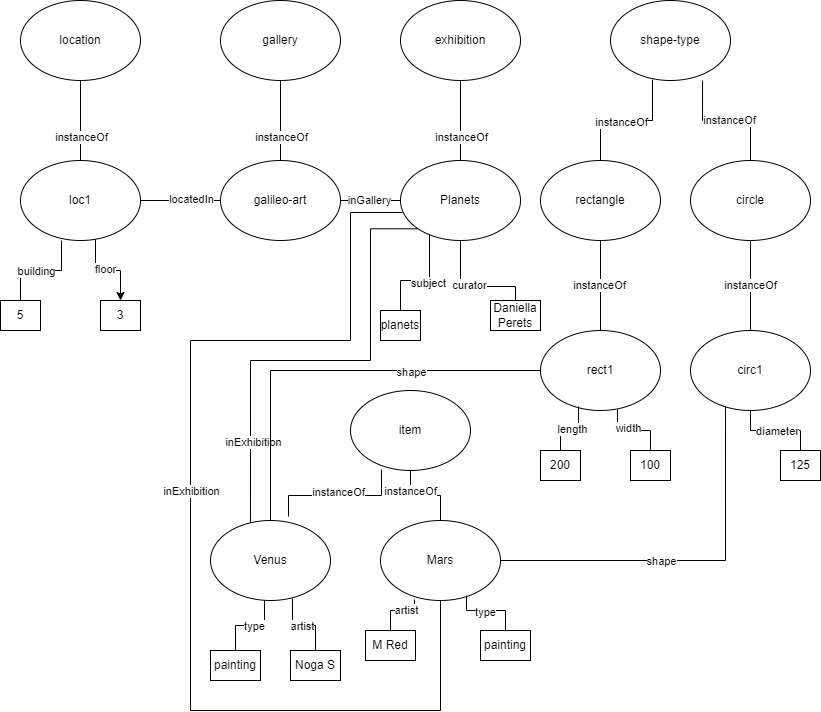
\includegraphics[width=0.7\linewidth]{meuseum.jpg}
\end{figure}

\pagebreak

\begin{hebrew}
    \section*{שאלה 2}
    \subsection*{סעיף א}

    נבצע את השאילתא הבאה:
\end{hebrew}

\begin{lstlisting}[language=SPARQL]
select ?kno, ?pname
where {
    ?kno instanceOf knesset
    ?kno kin ?rid
    ?pname pin ?rid
}
\end{lstlisting}

\begin{hebrew}
    \subsection*{סעיף ב}
    נבצע:
\end{hebrew}

\begin{lstlisting}[language=SPARQL]
select ?kno, ?pname
where {
    ?kno instanceOf knesset
    ?kno kin ?rid
    ?pname pin ?rid
}
\end{lstlisting}

\pagebreak

\begin{hebrew}

    \section*{שאלה 3}

    על פי הנתונים:

\end{hebrew}

\begin{align*}
     & n(d1,tables) =35                                   & n(d1,chairman)=15                            \\
     & TF(d1,tables) =\log(1+\frac{35}{250})=0.057        & n(d1, chairman)=\log(1+\frac{15}{250})=0.025 \\
     & IDF(tables)=0.25                                   & IDF(chairman)=0.167                          \\
     & TF-IDF(d1, Q)=0.057 * 0.25 + 0.025 * 0.167 = 0.018
\end{align*}

\begin{align*}
     & n(d2,tables) =10                                                     & n(d2,chairman)=30                            \\
     & TF(d2,tables) =\log(1+\frac{10}{250})=0.017                          & n(d1, chairman)=\log(1+\frac{30}{250})=0.049 \\
     & IDF(tables)=0.25                                                     & IDF(chairman)=0.167                          \\
     & TF-IDF(d2, Q)=0.017 * 0.25                   + 0.049 * 0.167 = 0.012
\end{align*}

\begin{hebrew}

    והמסמך d1 ידורג גבוה יותר במדד הרלוונטיות.

\end{hebrew}

\pagebreak

\begin{hebrew}
    \section*{שאלה 4}
    המטריצה T תיראה כך:
\end{hebrew}
\begin{align*}
    T=\begin{pmatrix}
          0 & 0.5 & 1 \\
          1 & 0   & 0 \\
          0 & 0.5 & 0
      \end{pmatrix}
\end{align*}
\begin{hebrew}
    אתחול: $P[1]\leftarrow 1/3, P[2]\leftarrow 1/3, P[3]\leftarrow 1/3$.
    באיטרציה הראשונה יתבצע:
\end{hebrew}

\begin{align*}
    P[1] & \leftarrow 0.06+ 0.82 * (0.5 * 1/3 + 1 * 1/3)=0.06 + 0.82 * 0.5 = 0.47 \\
    P[2] & \leftarrow 0.06 + 0.82 * (1 * 1/3)=0.333                               \\
    P[3] & \leftarrow 0.06 + 0.82 * (0.5 * 1/3) = 0.197
\end{align*}

\begin{hebrew}
    באיטרציה השנייה יתבצע:
\end{hebrew}

\begin{align*}
    P[1] & \leftarrow 0.06+ 0.82 * (0.5 * 0.333 + 1 * 0.197)=0.06 + 0.82 * 0.3635 = 0.358 \\
    P[2] & \leftarrow 0.06 + 0.82 * (1 * 0.47)=0.445                                      \\
    P[3] & \leftarrow 0.06 + 0.82 * (0.5 * 0.333) = 0.197
\end{align*}

\begin{hebrew}
    הדף המדורג באופן הנמוך ביותר יהיה דף 3
\end{hebrew}

\end{document}